\documentclass[10pt]{beamer}
\usepackage{verbatim}
\usepackage{amsmath}
\usepackage{amsthm}
\usepackage{graphics}
\usepackage{color}
\usepackage{algorithm, algorithmic}
\usepackage{stmaryrd}\usefonttheme[onlymath]{serif}

\title{Discussion 4: Experiment: Comparation to SVMRanker and LassoRanker}
\begin{document}

\maketitle
\begin{frame}\frametitle{Experiment Result}
\textbf{Experiment Configurations:}
Test cases are grabbed from data set of conference paper. Number of cases: 134.

Sampling Strategy: Lowerbound of number of points $=10$, expand sampling zone until reach the lowerbound.

Template Strategy: 
\begin{itemize}
\item Mulitphase: Linear templates: single variable plus linear combination of all.
\item SVMRanker: Linear + NonLinear
\item LassoRanker: Only Support Linear
\end{itemize}
\begin{center}
\begin{tabular}{|c|c|c|c|c|}
\hline
& 2-Multiphase& 5-Multiphase & SVMRanker & LassoRanker\\
\hline 
FINITE & 39 & 42&30 & 24\\
\hline 

INFINITE & 34& 34&34 & 37\\
\hline

UNKNOWN & 61& 58&70 & 73\\
\hline
TIME &1107s& 5709s& 162s& 1695s\\
\hline

\end{tabular}
\end{center}


Our algorithm can solve more cases than SVMRanker and LassoRanker.
\end{frame}


\begin{frame}\frametitle{Specifying Cases}
\begin{itemize}
\item Multiphase with depth 2 solved \& SVMRanker not solved:

$2,51,66,67,72,73,144,152,161$
\item SVMRanker solved \& Multiphase not solved:

$159$
\item Multiphase with depth 5 solved:

$7,155,126$
\item Advantage of Multiphase with depth 5 to LassoRanker:
$1,7,58,66,67,83,144,148,149,150,151,152,153,155,156,157$

$158,160,161,163,164,166,167,171$

\item LassoRanker's advantage to Multiphase:

Termination: $146,147,129,74,71,15$

Non-termination: $85,25,26$
\end{itemize}

\end{frame}



\begin{frame}\frametitle{Multiphase to SVMRanker}
We solve two types of new loops:
\begin{itemize}
\item Decreased by a variable: $2, 51,72,73,144,152,161$
\begin{center}
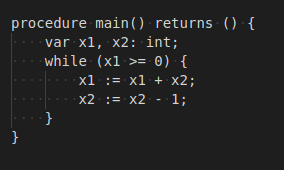
\includegraphics[scale=0.5]{2.png}
\end{center}
\item Flipping between negative and positive: $66,67$
\begin{center}
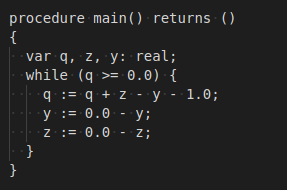
\includegraphics[scale=0.5]{66.png}
\end{center}
\end{itemize}
\end{frame}


\begin{frame}\frametitle{SVMRanker to Multiphase}
$159.bpl$

\begin{center}
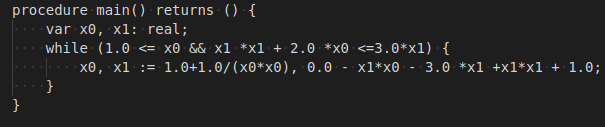
\includegraphics[scale=0.5]{159.png}
\end{center}Reason: we use the linear templates.
\end{frame}

\begin{frame}\frametitle{Multiphase with Depth 5}
$7,126$

\begin{center}
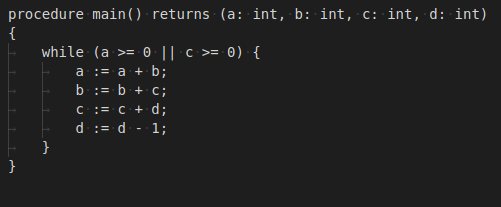
\includegraphics[scale=0.5]{7.png}
\end{center}

\end{frame}
\begin{frame}\frametitle{Continue}
$155$
\begin{center}
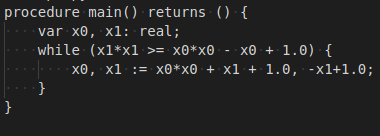
\includegraphics[scale=0.5]{155.png}

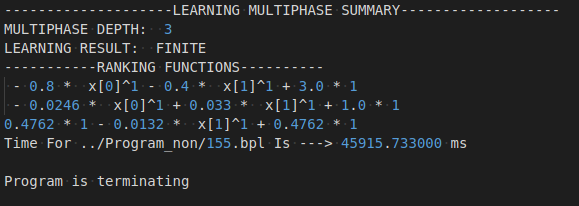
\includegraphics[scale=0.5]{155Result.png}
\end{center}
Not sure whether the result of this case is correct.

\end{frame}

\begin{frame}\frametitle{Termination: LassoRanker}
Termination: $146,147,129,74,71,15$
\begin{itemize}
\item $146,147$: large scale cases, where the number of variables is 51. Our algorithm goes timeout.
\item $129$: Might be the problem of incompatible types or redundant varibles. To be investigated later.
\begin{center}
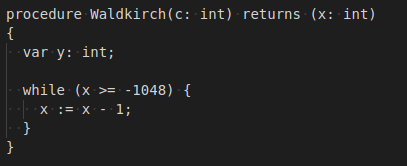
\includegraphics[scale=0.5]{129.png}
\end{center}
\item $74$
\begin{center}
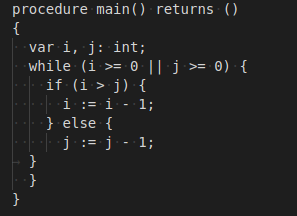
\includegraphics[scale=0.40]{74.png}
\end{center}
\end{itemize}
\end{frame}
\begin{frame}\frametitle{TODOs}
\begin{itemize}
\item Make the problems of cases above clear.
\item Do more experiment on different experiment configurations.
\item Write the experiment part of the paper.
\end{itemize}
\end{frame}
\end{document}
